\documentclass[a4paper,10pt]{article}
\usepackage[utf8]{inputenc}
\usepackage{amsmath}
\usepackage{amsfonts}
\usepackage{graphicx}
\usepackage{hyperref}
\usepackage{float}
\usepackage{caption}
\usepackage{tikz}
\usepackage{tabularx}
\usepackage{pgfplots}
\pgfplotsset{compat=1.15}
\usepackage{pgfplots}

\newcolumntype{Y}{>{\centering\arraybackslash}X}

\title{Options}
\author{Nathan NDJOLI - \href{mailto:nathan.ndjoli1@gmail.com}{nathan.ndjoli1@gmail.com}}
\date{July 2024}

\newcommand{\plotstrategy}[2]{
        \begin{figure}[H]
        \centering
        \begin{tikzpicture}
            \begin{axis}[
                x label style={anchor=east},
                y label style={anchor=south},
                xlabel=$St$,
                ylabel=Profit,
                grid=major,
                width=1\textwidth,
                height=0.4\textwidth,
                axis lines=middle,
                enlargelimits={abs=2},
                xtick=\empty,
                ytick={0},
                axis line style={very thin},
                ytick pos=left,
                xtick pos=bottom,
                domain=0:100,
                every axis y label/.style={at={(ticklabel cs:1.05)}, anchor=south},
                every axis x label/.style={at={(ticklabel cs:1.05)}, anchor=east},
                yticklabel style={anchor=west, font=\small},
                ]
                
                \addplot [
                    black,
                    thick
                ] table [x=S, y=Payoff, col sep=space] {#2};

            \end{axis}
        \end{tikzpicture}
        \caption{#1}
    \end{figure}
}


\begin{document}
\maketitle

\section*{Definition}

    \noindent Options are contracts between two parties where one grants the other the right to buy (call option) or sell (put option) an underlying asset in exchange for a premium. This purchase or sale occurs at a specified price (strike price) during a specific period or at a specific date called the expiration. \\
    
    \noindent As a conditional instrument, options can be based on various underlying assets such as stocks, indices, interest rates, currencies, or commodities. There are call options (calls) and put options (puts). The price of the option, called the premium, is denoted as \( C \) for a call and \( P \) for a put. The strike price is denoted as \( K \). When an option can be exercised at any time before expiration, it is called an American option. Conversely, if the option can only be exercised on a specific date, it is called a European option. \\
    
    \noindent For call options, they are said to be "in the money" when, at a moment \( t \), the price of the underlying asset \( S_t \) is greater than the strike price \( K \). They are "out of the money" if, at \( t \), \( S_t \) is less than \( K \). Finally, they are "at the money" when, at \( t \), \( S_t \) is equal to \( K \). \\
    
    \noindent For put options, the option is "in the money" if, at a moment \( t \), the price of the underlying asset \( S_t \) is less than the strike price \( K \). It is "out of the money" when, at \( t \), \( S_t \) is greater than \( K \). And it is "at the money" when, at \( t \), \( S_t \) is equal to \( K \). \\
    
\section*{Value of a European Option}

    \subsection*{Value at Expiration}

        \noindent The value of a European option at expiration is fundamentally tied to the relationship between the price of the underlying asset \( S_T \) and the strike price \( K \). For a call option, the value at expiration is captured by the formula:\\\[ C_T = \max(0, S_T - K) \]\\ This indicates that the call option holds value if the price of the underlying asset exceeds the strike price. Conversely, if the price of the underlying asset is less than or equal to the strike price, the value of the call option drops to zero. On the other hand, for a put option, the value at expiration is defined by \\\[ P_T = \max(0, K - S_T) \]\\ This implies that the put option holds value if the price of the underlying asset is below the strike price, and if it is higher or equal, the value becomes zero. \\
        
    \subsection*{Value at Time \( t \)}

        \noindent At any moment \( t \) before the expiration date, the value of an option comprises two distinct components: the intrinsic value and the time value. The intrinsic value is the value the option would have if it were at maturity at time \( t \). For a call option, the intrinsic value is calculated as: \\\[ C_{VI,t} = \max(0, S_t - K) \]\\ which reflects the positive difference between the current price of the underlying asset and the strike price, should it exist. For a put option, the intrinsic value is given by: \\\[ P_{VI,t} = \max(0, K - S_t) \]\\ which captures the positive difference between the strike price and the current price of the underlying asset. \\

        \noindent The time value of an option represents the additional value derived from the potential for the option to be exercised before its expiration date. This component acknowledges the uncertainty and potential variability in the price of the underlying asset over the remaining life of the option. As time progresses towards expiration, the time value diminishes, reflecting the decreasing uncertainty about the future price movements of the underlying asset. Consequently, the total value of an option at any time \( t \) is the sum of its intrinsic value and its time value, encapsulating both the immediate payoff and the speculative premium due to future price variability. \\
       
\section*{Examples of Option Usage}

    \noindent When an investor decides to buy a call option, he anticipates a rise in the price of the underlying asset. This strategy is known as a long call. If the underlying asset exceeds the strike price, the investor realizes unlimited profit, as he can buy the asset at the strike price and sell it at the higher market price. However, the potential loss is limited to the premium paid for the option.
        
        \plotstrategy{Long Call}{Long_Call.dat}
        
    \noindent Conversely, when an investor sells a call option, he hopes that the price of the underlying asset will remain below the strike price. This strategy, known as a short call, allows the investor to receive the option premium by betting that the option will not be exercised. However, if the asset price exceeds the strike price, the investor suffers potentially unlimited losses, as he will have to buy the asset at the higher market price to sell it at the lower strike price.\\
        
        \plotstrategy{Short Call}{Short_Call.dat}
        
    \noindent Regarding put options, buying a put option allows the investor to protect against a decline in the price of the underlying asset or to speculate on depreciation. This strategy, called a long put, generates potentially high profits if the asset price falls below the strike price, as the investor can sell the asset at the higher strike price. The loss is limited to the premium paid for the option.\\
        
        \plotstrategy{Long Put}{Long_Put.dat}
        
    \noindent Selling a put option, known as a short put, implies that the investor bets that the price of the underlying asset will remain above the strike price. The investor receives the option premium, hoping that it will expire worthless. However, if the asset price falls below the strike price, the investor must buy the asset at a price higher than the market price, resulting in losses that can be significant but limited to the strike price minus the premium received. \\
        
        \plotstrategy{Short Put}{Short_Put.dat}
        
    \noindent The straddle strategy consists of buying both a call option and a put option on the same underlying asset, with the same expiration and strike price. This approach is used to bet on significant volatility in the asset, regardless of the direction of the price movement. If the asset price changes significantly, the investor can realize substantial gains, either through the call option if the price rises or through the put option if the price falls. However, if the asset price remains stable, the investor loses the premiums paid for both options. \\
        
        \plotstrategy{Straddle}{Straddle.dat}
        
    \noindent The strangle, a similar strategy, also involves buying a call option and a put option on the same underlying asset but with different strike prices and the same expiration date. The call option's strike price is higher than the current market price of the asset, while the put option's strike price is lower than the current market price. This strategy profits from significant movements in either direction, with losses limited to the premiums paid if prices remain stable. The figure "Strangle Profit/Loss" shows this setup. \\

        \plotstrategy{Strangle}{Strangle.dat}
        
    \noindent The bull spread is an options strategy that involves buying a call option with a strike price \( K_1 \) and selling a call option with a strike price \( K_2 \) (where \( K_2 > K_1 \)), both on the same asset and with the same expiration. This approach allows for limiting both potential gains and losses. The maximum profit is achieved if the asset price exceeds \( K_2 \), and the maximum loss occurs if the price remains below \( K_1 \). \\
       
        \plotstrategy{Bull Spread}{Bull_Spread.dat}
        
    \noindent The butterfly spread combines bullish and bearish spreads with fixed risk and profit. It typically involves buying one option at a lower strike price \( K_1 \), selling two options at a middle strike price \( K_2 \), and buying one option at a higher strike price \( K_3 \). The strike prices are equidistant. This strategy benefits when the asset price remains close to \( K_2 \) at expiration. Gains and losses are limited, as shown in the figure. \\

        \plotstrategy{Butterfly Spread}{Butterfly_Spread.dat}

    \noindent Finally, the iron condor is a strategy composed of four different options with the same expiration. It combines a bear call spread and a bull put spread on the same underlying asset. The bear call spread involves selling a call option at a lower strike price \( K_2 \) and buying a call option at a higher strike price \( K_3 \). The bull put spread involves selling a put option at a higher strike price \( K_1 \) and buying a put option at a lower strike price \( K_4 \). This strategy aims to profit from low volatility in the asset price, hoping that the price will stay between \( K_1 \) and \( K_2 \) at expiration. Gains and losses are limited. \\
        
        \plotstrategy{Iron Condor}{Iron_Condor.dat}
        
\section*{The Call/Put Parity Relationship}

    \subsection*{Analysis Framework}

        \noindent To understand the parity relationship between a call and a put, we consider a framework where the securities are divisible, the risk-free rate is continuous and denoted as \( i \), and there are no arbitrage opportunities or frictions (no transaction costs, taxes, or financial constraints). We focus on European options on underlying assets that do not pay any intermediate income.
        
    \subsection*{Relationship Between Call \& Put value}

        \noindent The objective is to demonstrate that there is a relationship between a call and a put with the same expiration and the same underlying asset. This relationship is illustrated by the following equation:
        \\\[ C_t + K e^{-i(T-t)} = P_t + S_t \]\\
        \noindent For a portfolio composed of a call and an amount \( K e^{-i(T-t)} \) invested at the risk-free rate, it must be equivalent to a portfolio composed of a put and the underlying asset.
        
    \subsection*{Demonstration}

        \noindent If the equation \( C_t + K e^{-i(T-t)} > P_t + S_t \) holds, there is an arbitrage opportunity by selling portfolio 1 (call and investment) and buying portfolio 2 (put and underlying asset). The cash flows at time \( t \) show a risk-free profit, which is not possible in an efficient market. \\
        
        \noindent Conversely, if the equation \( C_t + K e^{-i(T-t)} < P_t + S_t \) holds, there is an arbitrage opportunity by buying portfolio 1 and selling portfolio 2, thus realizing an immediate and risk-free profit.
        
    \subsection*{Comments}

        \noindent The call/put parity relationship allows synthesizing or duplicating a call from a risk-free security (loan), the underlying asset, and a put, and vice versa for a put. This relationship is fundamental for arbitrage and portfolio management of options, ensuring market efficiency.
        
\section*{The Cox, Ross, and Rubinstein (1979) Model}

    \noindent The Cox, Ross, and Rubinstein (1979) model is a simplified method for evaluating options, published in the Journal of Financial Economics. This model, often referred to as the binomial model, offers an intuitive approach to determining the price of options using binomial trees.
    
    \subsection*{Analysis Framework}
    
        \noindent The general assumptions of the model include the divisibility of securities, the absence of arbitrage opportunities, the absence of frictions such as transaction costs or taxes, and the use of a discrete risk-free rate, denoted as \( r \). We consider a European option with a one-period expiration and an underlying asset that does not pay any intermediate income.
    
    \subsection*{Binomial Trees}
    
        \noindent The model uses a binomial tree to represent the different possible trajectories of the underlying asset's price. During the option's life period, the initial value of the underlying asset, denoted \( S_0 \), can be multiplied by \( u \) (where \( u > 1 \)) with a probability \( p \), or by \( d \) (where \( 0 < d < 1 \)) with a probability \( 1 - p \). At the end of the period, the value of the call will be denoted \( C_u \) in case of an increase and \( C_d \) in case of a decrease.
        
        \begin{figure}[ht]
        \centering
        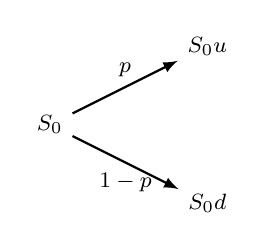
\begin{tikzpicture}[scale=2, font=\footnotesize]
            % Nodes
            \node (S0) at (0,0) {$S_0$};
            \node (Su) at (1,0.5) {$S_0u$};
            \node (Sd) at (1,-0.5) {$S_0d$};
        
            % Lines
            \draw[thick, -latex] (S0) -- (Su) node[midway, above] {$p$};
            \draw[thick, -latex] (S0) -- (Sd) node[midway, below] {$1-p$};
        \end{tikzpicture}
        \caption{One-period binomial tree for the CRR model}
        \end{figure}
        
    \subsection*{Determination of the Call Value}
    
        \noindent To determine the value of a call, we construct a risk-free portfolio consisting of the purchase of a call and the sale of a fraction \( \Delta \) of the underlying asset. The initial value of the portfolio is given by \( W_0 = C - \Delta S_0 \), and the value of the portfolio at expiration will be:
        \\\[ 
        \begin{cases} 
        W_T = C_u - \Delta u S_0 & \text{in case of an increase} \\
        W_T = C_d - \Delta d S_0 & \text{in case of a decrease}
        \end{cases} 
        \]\\
        
        \begin{figure}[ht]
        \centering
        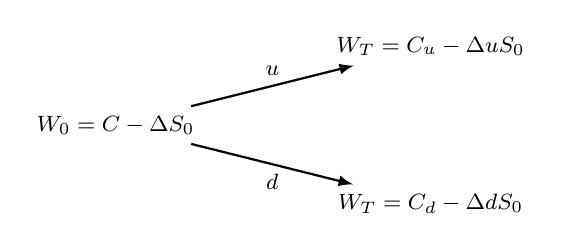
\begin{tikzpicture}[scale=2, font=\footnotesize]
            % Nodes
            \node (S0) at (0,0) {$W_0 = C - \Delta S_0$};
            \node (Su) at (2,0.5) {$W_T = C_u - \Delta u S_0$};
            \node (Sd) at (2,-0.5) {$W_T = C_d - \Delta d S_0$};
        
            % Lines
            \draw[thick, -latex] (S0) -- (Su) node[midway, above] {$u$};
            \draw[thick, -latex] (S0) -- (Sd) node[midway, below] {$d$};
        \end{tikzpicture}
        \caption{Determination of call value in a risk-neutral world}
        \end{figure}
        
        \noindent The return of the portfolio must be the same regardless of the scenario, allowing us to solve for \( \Delta \) and ultimately determine the value of the call:
        \\\[ 
        \Delta = \frac{C_u - C_d}{S_0 (u - d)} 
        \]\\.
        \\\[ 
        C = \frac{C_u (1 + r - d) - C_d (1 + r - u)}{(1 + r)(u - d)} 
        \]\\
        
    \subsection*{Extensions}
    
        \noindent The model can be extended to handle put options and options with multiple periods. For a put, the expression is:
        \\\[ P = \frac{P_u (1 + r - d) - P_d (1 + r - u)}{(1 + r)(u - d)} \]\\
        
        \noindent Models with multiple periods use a backward induction approach to determine the option's value at each node of the binomial tree.
        
        \begin{figure}[H]
        \centering
        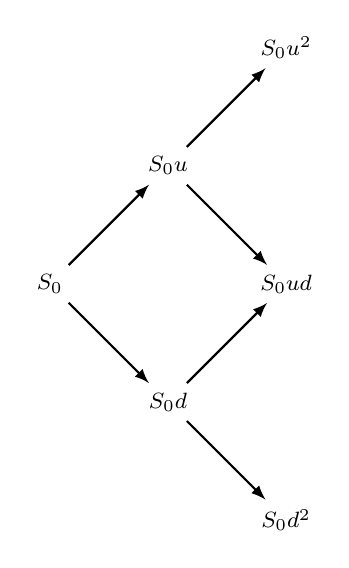
\begin{tikzpicture}[scale=1.5, font=\footnotesize]
            % Nodes at time 0
            \node (S0) at (0,0) {$S_0$};
        
            % Nodes at time 1
            \node (Su1) at (1,1) {$S_0u$};
            \node (Sd1) at (1,-1) {$S_0d$};
        
            % Nodes at time 2
            \node (Su2) at (2,2) {$S_0u^2$};
            \node (Sud) at (2,0) {$S_0ud$};
            \node (Sd2) at (2,-2) {$S_0d^2$};
        
            % Lines
            \draw[thick, -latex] (S0) -- (Su1);
            \draw[thick, -latex] (S0) -- (Sd1);
            \draw[thick, -latex] (Su1) -- (Su2);
            \draw[thick, -latex] (Su1) -- (Sud);
            \draw[thick, -latex] (Sd1) -- (Sud);
            \draw[thick, -latex] (Sd1) -- (Sd2);
        \end{tikzpicture}
        \caption{Multiple-period binomial model}
        \end{figure}
        
    \subsection*{American Option Case}
    
        \noindent American options, which can be exercised at any time before expiration, require calculations at each intermediate node of the binomial tree. For each node, two values are calculated: the option's value if it is not exercised and its value if it is exercised (as if the date in question were the expiration). The higher of the two values is then retained for each node.
        
        \begin{figure}[H]
        \centering
        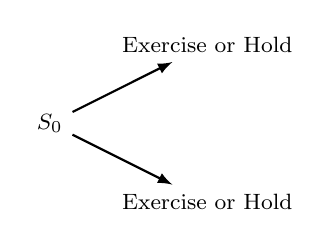
\begin{tikzpicture}[scale=2, font=\footnotesize]
            % Nodes
            \node (S0) at (0,0) {$S_0$};
            \node (Su) at (1,0.5) {Exercise or Hold};
            \node (Sd) at (1,-0.5) {Exercise or Hold};
        
            % Lines
            \draw[thick, -latex] (S0) -- (Su);
            \draw[thick, -latex] (S0) -- (Sd);
        \end{tikzpicture}
        \caption{Decision nodes for an American option}
        \end{figure}
        
\section*{The Black-Scholes Model}

    \noindent The Black-Scholes model, published in 1973, is a fundamental method for evaluating options and corporate liabilities. It is described in the article "The Pricing of Options and Corporate Liabilities" in the Journal of Political Economy.\\
    
    \noindent The Black-Scholes model determines the price of options in continuous time, using stochastic processes. The price of the underlying asset is assumed to follow a log-normal distribution, and the volatility of the underlying asset's price is denoted \( \sigma \).\\
    
    
    \noindent The value of a call (\( C_t \)) and a put (\( P_t \)) in this model is given by the following formulas:\\
    \\\[ C_t = S_t N(d1) - K e^{-r(T-t)} N(d2) \]\\
    \\\[ P_t = -S_t N(-d1) + K e^{-r(T-t)} N(-d2) \]\\
    
    \noindent Where:\\
    \\\[ d1 = \frac{\ln \left( \frac{S_t}{K} \right) + (T-t) \left( r + \frac{\sigma^2}{2} \right)}{\sigma \sqrt{T-t}} \]\\
    \\\[ d2 = \frac{\ln \left( \frac{S_t}{K} \right) + (T-t) \left( r - \frac{\sigma^2}{2} \right)}{\sigma \sqrt{T-t}} \]\\
    
    \noindent Note: \( d2 = d1 - \sigma \sqrt{T-t} \).\\
    
    \noindent When the underlying asset pays a continuous dividend at rate \( g \), the formulas are adjusted as follows:\\
    \\\[ C_t = S_t e^{-g(T-t)} N(d1) - K e^{-r(T-t)} N(d2) \]\\
    \\\[ P_t = -S_t e^{-g(T-t)} N(-d1) + K e^{-r(T-t)} N(-d2) \]\\
    
    \noindent Where:\\
    \\\[ d1 = \frac{\ln \left( \frac{S_t}{K} \right) + (T-t) \left( r - g + \frac{\sigma^2}{2} \right)}{\sigma \sqrt{T-t}} \]\\
    \\\[ d2 = \frac{\ln \left( \frac{S_t}{K} \right) + (T-t) \left( r - g - \frac{\sigma^2}{2} \right)}{\sigma \sqrt{T-t}} \]\\

    \noindent If the underlying asset pays a discrete dividend \( D \) at a date \( t' \) (between \( t \) and \( T \)), the present value of the dividend at \( t \) is denoted \( D' \). The formulas become:\\
    \\\[ C_t = (S_t - D') N(d1) - K e^{-r(T-t)} N(d2) \]\\
    \\\[ P_t = -(S_t - D') N(-d1) + K e^{-r(T-t)} N(-d2) \]\\
    
    \noindent Where:\\
    \\\[ d1 = \frac{\ln \left( \frac{S_t - D'}{K} \right) + (T-t) \left( r + \frac{\sigma^2}{2} \right)}{\sigma \sqrt{T-t}} \]\\
    \\\[ d2 = \frac{\ln \left( \frac{S_t - D'}{K} \right) + (T-t) \left( r - \frac{\sigma^2}{2} \right)}{\sigma \sqrt{T-t}} \]\\
    
\section*{Greeks}

    \subsection*{Delta}
        \noindent Delta represents the first derivative of the option price with respect to the price of the underlying asset. For a call option, delta is given by:\\\[ \Delta C = \frac{\partial C_t}{\partial S_t} = N(d1) \]\\ And for a put option, it is defined as: \\\[ \Delta P = \frac{\partial P_t}{\partial S_t} = N(d1) - 1 \]\\ Delta measures the rate of change in the option price per unit change in the price of the underlying asset, indicating how much the option price will move if the underlying asset's price changes by one unit. The delta of a call is always positive, ranging between 0 and 1, reflecting the increasing value of the call option as the price of the underlying asset increases. Conversely, the delta of a put is always negative, ranging between -1 and 0, which signifies that the value of the put option decreases as the price of the underlying asset rises. Notably, the delta of the underlying asset itself is equal to 1. \\
    
    \subsection*{Gamma}
        \noindent Gamma, on the other hand, is the second derivative of the option price with respect to the price of the underlying asset. It is calculated as:\\\[ \Gamma = \frac{\partial^2 C_t}{\partial S_t^2} = \frac{\partial^2 P_t}{\partial S_t^2} = \frac{N'(d1)}{S_t \sigma \sqrt{T-t}} \]\\ Gamma measures the rate of change of delta with respect to changes in the underlying asset's price, reflecting the convexity of the option's value in relation to the price movements of the underlying asset. A high gamma indicates that delta can change significantly with even small movements in the underlying asset's price. Gamma is always positive for options, meaning that as the price of the underlying asset changes, the rate of change of delta also increases. This property is at its maximum when the option is at the money. Additionally, the gamma of the underlying asset is always zero, indicating no change in delta with respect to price movements. \\
    
    \subsection*{Theta}
        \noindent Theta is the first derivative of the option price with respect to time. It represents the rate at which the option's value decreases as it approaches expiration. For a call option, theta is given by:\\\[ \Theta C = \frac{\partial C_t}{\partial t} = -\frac{S_t \sigma N'(d1)}{2 \sqrt{T-t}} - r K e^{-r(T-t)} N(d2) \]\\ And for a put option, it is:\\\[ \Theta P = \frac{\partial P_t}{\partial t} = -\frac{S_t \sigma N'(d1)}{2 \sqrt{T-t}} + r K e^{-r(T-t)} N(-d2) \]\\ Theta essentially captures the time decay of an option, reflecting the decrease in value as the expiration date approaches. The theta of a call is always negative, indicating the erosion of the option's value over time. Theta is very low when the option is out of the money and reaches its maximum when the option is at the money. \\
    
    \subsection*{Vega}   
    
        \noindent Vega measures the sensitivity of the option price to changes in the volatility of the underlying asset. It is defined as:\\\[ \nu = \frac{\partial C_t}{\partial \sigma} = \frac{\partial P_t}{\partial \sigma} = S_t \sqrt{T-t} N'(d1) \]\\ Vega indicates how much the price of the option will change with a 1\%\ change in the implied volatility of the underlying asset, making it a crucial measure for understanding the impact of market volatility on option prices. Vega is always positive for options, indicating that higher volatility increases the option's value. However, the vega of the underlying asset is zero. Moreover, vega decreases as time passes and reaches its maximum when the option is at the money. \\
    
    \subsection*{Rho}    
    
        \noindent Rho is the first derivative of the option price with respect to the interest rate. For a call option, rho is given by:\\\[ \rho C = \frac{\partial C_t}{\partial r} = K (T-t) e^{-r(T-t)} N(d2) \]\\ And for a put option, it is:\\ \\\[ \rho P = \frac{\partial P_t}{\partial r} = -K (T-t) e^{-r(T-t)} N(-d2) \]\\ Rho measures the sensitivity of the option price to changes in the interest rate, reflecting how the present value of the strike price is affected by interest rate fluctuations. The rho of a call is always positive, indicating that an increase in interest rates will increase the value of the call option. Conversely, the rho of a put is always negative, suggesting that an increase in interest rates will decrease the value of the put option. \\
    
    \subsection*{Greeks in Portfolio Management} 
    
        \noindent In practical terms, delta is used to hedge against changes in the price of the underlying asset. This is achieved by buying or selling the underlying asset to offset the changes in the value of the options held in the portfolio. For instance, a delta-neutral portfolio is constructed by ensuring that the overall delta of the portfolio is zero. This means buying a call option and selling a specific number of units of the underlying asset such that the portfolio’s delta, \(\Delta_C - x \Delta_S\), equals zero, where \(x\) is the number of units of the underlying asset sold. \\
        
        \noindent Gamma and vega hedging are more sophisticated strategies that involve trading options rather than the underlying asset itself. Gamma measures the rate of change of delta with respect to the price of the underlying asset, reflecting the curvature or convexity of the option’s value relative to price movements. A gamma-neutral portfolio is one where the gamma is balanced, meaning the portfolio’s sensitivity to changes in delta is minimized. This is achieved by determining \(x\) such that the gamma of the whole portfolio, \(\Gamma_W + x \Gamma_O\), equals zero. Vega, on the other hand, measures the sensitivity of the option price to changes in the volatility of the underlying asset. A vega-neutral portfolio ensures that the portfolio’s value is not affected by changes in volatility. \\
        
        \noindent In some scenarios, managing portfolio risks might require using more than one option to achieve neutrality in both gamma and vega. This involves determining the quantities \(x_1\) and \(x_2\) of two different options, \(O1\) and \(O2\), respectively, such that both the gamma and vega of the portfolio are neutralized. Mathematically, this can be expressed as solving the system of equations:
        \[
        \begin{cases} 
        \Gamma_W + x_1 \Gamma_{O1} + x_2 \Gamma_{O2} = 0 \\
        \nu_W + x_1 \nu_{O1} + x_2 \nu_{O2} = 0 
        \end{cases}
        \]
        Here, \(\Gamma_W\) and \(\nu_W\) represent the gamma and vega of the existing portfolio, while \(\Gamma_{O1}\), \(\Gamma_{O2}\), \(\nu_{O1}\), and \(\nu_{O2}\) are the gamma and vega values of the two options being considered. This approach ensures that the portfolio is effectively hedged against both gamma and vega risks, maintaining a stable value despite fluctuations in the underlying asset's price and its volatility. \\


\end{document}
